% =============================================================================
% ECTI Transactions on Computer and Information Technology (ECTI-CIT)
% Two-column eec_style class (10pt). Length target 8-12 pages.
% Double-blind: author identity withheld for review.
%
% "Discard the Arrow, Keep the Drift": a Mincer-Zarnowitz efficiency analysis and
% shrinkage correction of a deployed equity-return forecaster.
%
% Every number is a measured statistic from the authors' append-only forecast
% ledger (619 resolved forecasts, 2026-04-19 to 2026-06-12). Figures are
% generated directly from that ledger.
% =============================================================================
\documentclass[10pt,twocolumn,twoside]{eec_style}
\usepackage{graphicx}
\usepackage{amsmath,amssymb,amsbsy}
\usepackage{booktabs}
\usepackage{multirow}
\usepackage{array}
\usepackage{url}
\usepackage{bm}
\usepackage[dvipsnames]{xcolor}
\usepackage{mathtools}
\usepackage{algorithm}
\usepackage{algorithmic}

\graphicspath{{figures/}}
\DeclareGraphicsExtensions{.pdf,.png,.eps}
\newcommand{\fig}[1]{Fig.~\ref{fig:#1}}
\newcommand{\tab}[1]{Table~\ref{tab:#1}}
\newcommand{\refsec}[1]{Section~\ref{sec:#1}}
\newtheorem{definition}{Definition}
\newtheorem{proposition}{Proposition}

\title{When the Forecast Loses to No-Change: Point-Forecast Inefficiency and a
Shrink-to-Drift Correction in a Deployed Equity-Return Model}

% NOTE: ECTI-CIT review is double-blind; for the anonymous review copy, remove the
% author block and the affiliation footnote below.
\authorlist{%
 \authorentry{Anandkumar Pardeshi\( ^{1,\ast} \)}{}{}
 \authorentry{Sujata Deshmukh\( ^{2} \)}{}{}
}
\received{2026}{6}{29}{2026}{6}{29}
\runninghead{Point-Forecast Inefficiency in a Deployed Equity-Return Model}
\setcounter{page}{1}

\begin{document}
\maketitle

\begin{abstract}
A machine-learning forecaster that is deployed to predict returns makes an implicit
promise: its point forecast is the conditional mean, so acting on the forecast should
beat ignoring it. We test that promise directly on an append-only, point-in-time
ledger of $619$ resolved forecasts from a production equity-forecasting service for
liquid Indian (NSE) equities, in which every median return forecast was recorded
before its outcome was known. A Mincer--Zarnowitz efficiency regression of realized
on forecast return yields a slope of $-0.23$ (bootstrap $95\%$ interval
$[-0.35,-0.12]$), which excludes both the value $1$ demanded of an efficient forecast
and the value $0$ of a useless one: the forecasts are not merely uninformative, they
are \emph{perversely signed}. The signature is over-extrapolation --- the most bullish
forecast decile ($+5.5\%$ mean predicted) realizes $-1.3\%$, and directional accuracy
is $46.4\%$, below a coin. We then derive the error-minimizing linear response, a
single shrinkage coefficient applied to the forecast, and estimate it walk-forward.
The optimal coefficient is $k^\star\approx 0$ (interval $[-0.33,0.09]$), i.e.\ the
loss-minimizing action is to \emph{discard the forecast's directional content and
predict the drift}. Doing so cuts out-of-sample root-mean-square error from $0.053$ to
$0.031$ --- a $66\%$ reduction in mean-squared error --- and the improvement is
significant by a Diebold--Mariano test (statistic $6.4$), whereas the residual gain of
the optimally-shrunk forecast over the plain drift baseline is not ($1.8$). The
contribution is a small, reusable diagnosis-and-correction method: measure forecast efficiency
on a leakage-free ledger, and when the efficiency test fails, route only the parts of
the system that carry information --- here, the drift and the calibrated uncertainty ---
rather than the point forecast's direction. The result is also a cautionary tale for
applied forecasting: a model can post plausible point predictions while its directional
content is worse than worthless, and only an efficiency analysis reveals it.
\end{abstract}

\begin{keywords}
Forecast evaluation, Mincer--Zarnowitz regression, over-extrapolation, shrinkage
estimation, machine learning deployment, financial forecasting, model diagnostics.
\end{keywords}

\footnotetext{\hspace{2mm}\( ^{1} \)Department of Computer Science and Engineering, Fr.\ C.\ Rodrigues Institute of Technology, University of Mumbai, Navi Mumbai 400703, India.}
\footnotetext{\hspace{2mm}\( ^{2} \)Department of Computer Engineering, Fr.\ C.\ Rodrigues Institute of Technology, University of Mumbai, Navi Mumbai 400703, India.}
\footnotetext{\hspace{2mm}\( ^{\ast} \)Corresponding author. E-mail: anand.pardeshi@fcrit.ac.in. ORCID: 0000-0002-1825-0097 (Pardeshi), 0000-0001-5109-3700 (Deshmukh).}

% =============================================================================
\section{Introduction}
\label{sec:intro}
% =============================================================================
When a machine-learning system is deployed to forecast a continuous quantity --- a
demand, a price, a return --- and a human or an automated policy then acts on that
forecast, the system makes an implicit statistical promise. It promises that its point
output is, to a useful approximation, the conditional mean of the target given the
information available. If the promise holds, the forecast is \emph{efficient}: no
linear reweighting of it can reduce expected squared error, and acting on it beats
ignoring it. If the promise fails, the forecast can still look entirely reasonable ---
plausible magnitudes, sensible direction --- while being, in the precise sense we make
below, worse than useless.

This paper reports an efficiency analysis of a deployed equity-return forecaster and a
small correction that follows from it. The system serves liquid Indian (NSE) equities and,
at each decision time, emits a median return forecast at a fixed horizon, which it
writes to an append-only ledger before the outcome is known. Two months of operation
left $619$ resolved forecasts whose predicted and realized returns we can compare
without any possibility of look-ahead leakage, because the predictive fields were
sealed at issue time and the realized outcome was joined later. This is the right
substrate for an efficiency test: the classical regression of realized on forecast
value \cite{mincer1969,theil1966} is only meaningful when the forecasts were genuinely
made in advance, which a backtest cannot guarantee but a write-once ledger can.

The analysis returns an unusually sharp verdict. The Mincer--Zarnowitz slope of realized
on forecast return is $-0.23$, with a bootstrap $95\%$ interval of $[-0.35,-0.12]$
that excludes both endpoints of interest: it is not $1$ (the forecasts are
inefficient) and it is not $0$ (they are not merely noise). A negative slope means the
forecasts are \emph{perversely signed} --- on average the realized return moves against
the prediction. The mechanism is over-extrapolation, a pattern long documented in human
and model expectations \cite{bordalo2019}: the more boldly the system
predicts a move, the more the subsequent return disappoints, until the most bullish
forecast decile (mean prediction $+5.5\%$) realizes $-1.3\%$. Directional accuracy is
$46.4\%$, below the $50\%$ of a coin flip.

What should a practitioner do with such a forecaster? The temptation is to retrain, but
that presumes the architecture can extract a directional edge that, in a near-efficient
market \cite{fama1970,welch2008}, may simply not be there to extract. We take a
different and more conservative route. We ask: among all linear transforms of the
forecast, which minimizes deployed error? The answer is a single shrinkage coefficient,
and on this system it is statistically indistinguishable from zero. The
loss-minimizing action is therefore to \emph{stop using the forecast's directional
content} and to predict the drift instead. This is not a counsel of despair but a
concrete, validated deployment change: it cuts out-of-sample root-mean-square error by
a third (a $66\%$ reduction in mean-squared error), and the improvement is significant
under a Diebold--Mariano test \cite{diebold1995}, whereas the extra complexity of an
optimally-tuned shrinkage buys nothing over the plain drift baseline.

Our contributions are:
\begin{enumerate}
\item \textbf{An efficiency analysis on a leakage-free ledger.} We apply the
Mincer--Zarnowitz test, directional accuracy, and a binned reliability curve to a
production forecaster's point predictions, recorded point-in-time, and document a
significantly negative efficiency slope --- over-extrapolation severe enough to invert
the forecast's sign (\refsec{diagnosis}).
\item \textbf{A shrinkage correction with a stated optimum.} We derive the
error-minimizing shrinkage coefficient, show it is indistinguishable from zero on this
system, and interpret the result as a deployment rule: discard the arrow, keep the
drift (\refsec{shrink}).
\item \textbf{An honest out-of-sample validation.} Walk-forward Diebold--Mariano tests
and bootstrap intervals establish that drift significantly beats the raw forecast and
that nothing significantly beats drift, so the simplest correction is also the best the
data support (\refsec{results}).
\end{enumerate}
We are deliberate about scope: the analysis characterizes one deployment over one
two-month, six-name window, and we claim nothing beyond it (\refsec{threats}). But the
\emph{method} --- and the discipline of checking forecast efficiency before trusting a
deployed point prediction --- is general, and the failure it exposes is, we suspect,
more common in applied forecasting than the literature's focus on accuracy metrics
would suggest.

% =============================================================================
\section{Related Work}
\label{sec:related}
% =============================================================================
\textbf{Forecast efficiency and rationality.} The regression of the realized value on
the forecast, with a test of unit slope and zero intercept, is the classical efficiency
and unbiasedness test of Mincer and Zarnowitz \cite{mincer1969}, building on Theil
\cite{theil1966}. A forecast passes only if it leaves no linearly exploitable structure
in its own errors. Comparative accuracy of competing forecasts is tested by Diebold and
Mariano \cite{diebold1995}; we use both tools, the first to diagnose and the second to
validate the correction. These instruments are standard in econometric forecasting yet are
rarely turned on the point outputs of deployed machine-learning systems, which are
usually reported through error magnitudes (RMSE, MAE) or directional accuracy alone ---
summaries that, as we show, can look acceptable while the efficiency test fails
catastrophically.

\textbf{Over-extrapolation in expectations.} That forecasters, human and algorithmic,
over-react to recent or salient information and extrapolate it too far is documented
across survey expectations and asset prices \cite{bordalo2019,greenwood2014}.
A diagnostic-expectations model predicts exactly the pattern we observe: bold forecasts
are followed by systematic reversal, producing a negative slope of realized on forecast
\cite{bordalo2018}. Our contribution here is empirical and operational --- we measure the
effect in a live system's recorded outputs and turn the measurement into a deployment
decision --- rather than a new behavioral model.

\textbf{Return predictability and its limits.} A large literature is skeptical that
out-of-sample equity-return prediction beats simple benchmarks: Welch and Goyal find
that many predictors fail to outperform the historical mean out of sample
\cite{welch2008}, while Campbell and Thompson argue that small, constrained gains are
possible \cite{campbell2008}. Machine-learning asset-pricing models report
predictability under careful protocols \cite{gu2020}, but the methodological literature
warns repeatedly about backtest overfitting and look-ahead leakage
\cite{bailey2014,lopez2018}. Our finding sits comfortably inside this debate: on this
deployment, the conservative benchmark (drift) wins, and we make the case
quantitatively rather than by assertion.

\textbf{Calibration versus efficiency.} A forecaster can be well calibrated yet
inefficient, and conversely. Calibration concerns whether stated uncertainties match
realized frequencies --- whether a $90\%$ interval covers $90\%$ of the time --- and is
corrected by rescaling probabilities or interval widths. Efficiency concerns whether the
\emph{point} forecast is the conditional mean, and is corrected by reweighting the
forecast itself. The two are orthogonal: widening an interval does nothing to a
mis-signed point forecast, and shrinking a point forecast does nothing to an
overconfident band. The present paper addresses the efficiency side, which a
calibration fix leaves untouched. We stress the distinction because a practitioner who
has fixed calibration may wrongly believe the forecast is now trustworthy to act on,
when an efficiency test would reveal that its direction should be discarded.

\textbf{Shrinkage estimation.} Shrinking an estimator toward a prior reduces
mean-squared error when the estimator is noisy, a principle that runs from Stein and
James--Stein \cite{stein1956,james1961} through ridge regression \cite{hoerl1970} to
modern combination-of-forecasts work \cite{timmermann2006}. Our correction is the simplest
instance: a scalar shrinkage of a single forecast toward the drift, with the
shrinkage chosen to minimize squared error. The novelty is not the estimator but the
diagnosis that drives it to its degenerate optimum --- shrink all the way --- and the
walk-forward evidence that the degenerate optimum is the right operating point.

% =============================================================================
\section{System and Evaluation Ledger}
\label{sec:system}
% =============================================================================
The service under study issues, for an instrument with price $P_t$ at decision time $t$, a
median price forecast $\hat{P}_{t+h}$ at horizon $h$ trading days. We work in returns:
the \emph{forecast return} $f_t=(\hat{P}_{t+h}-P_t)/P_t$ and the \emph{realized return}
$r_t=(P_{t+h}-P_t)/P_t$. The point forecast is produced by a hybrid ensemble; its
internals are irrelevant to the analysis, which treats the forecaster as a black box that
emits $f_t$ and asks whether $f_t$ is an efficient predictor of $r_t$.

Every forecast is written at issue time to a write-once ledger row (instrument,
timestamp, horizon, anchor price, median forecast, model version); when the horizon
elapses, a resolution pass joins the realized price. Because the predictive fields are
immutable and sealed before the outcome exists, the ledger cannot leak future
information into the evaluation --- the property that makes an efficiency test credible.
We analyze the $619$ resolved forecasts issued between 19~April and 12~June~2026 across
six instruments, dominated by the ten-day horizon. Forecast returns have mean $1.7\%$
and standard deviation $2.3\%$; realized returns have mean $-0.2\%$ and standard
deviation $4.1\%$. The forecasts are thus systematically more optimistic and less
dispersed than reality, a first hint of the inefficiency we now quantify. To our
knowledge, the efficiency of this kind of deployed point forecast --- in the
Mincer--Zarnowitz sense, on a live point-in-time ledger --- has not previously been
tested, and the shrink-to-drift correction that follows from it is the contribution that
licenses the deployment recommendation of \refsec{discussion}.

% =============================================================================
\section{Efficiency Diagnosis}
\label{sec:diagnosis}
% =============================================================================
\subsection{The Mincer--Zarnowitz test}
We regress realized return on forecast return,
\begin{equation}
r_t = a + b\, f_t + \varepsilon_t,
\label{eq:mz}
\end{equation}
and test the joint efficiency hypothesis $(a,b)=(0,1)$ \cite{mincer1969}. The fitted
values are $a=0.0024$ (standard error $0.0020$; not distinguishable from zero) and
\begin{equation}
\hat b = -0.233\ (\text{s.e.}\ 0.070),\qquad
t_{b=1} = -17.6,\quad t_{b=0} = -3.3 .
\end{equation}
The slope is rejected against the efficient value $1$ with overwhelming force, and ---
the striking part --- it is also significantly \emph{below} zero. A bootstrap over
forecasts ($2000$ resamples) gives a $95\%$ interval for $b$ of $[-0.353,-0.115]$,
which excludes zero. The regression $R^2$ is $0.018$. In words: the forecasts explain
almost none of the variance of realized returns, and what little linear relationship
exists points the \emph{wrong way}. \fig{mz} plots the cloud, the fitted line (slope
$-0.23$), and the $45^\circ$ efficient line for reference.

\begin{figure*}[!t]
\centering
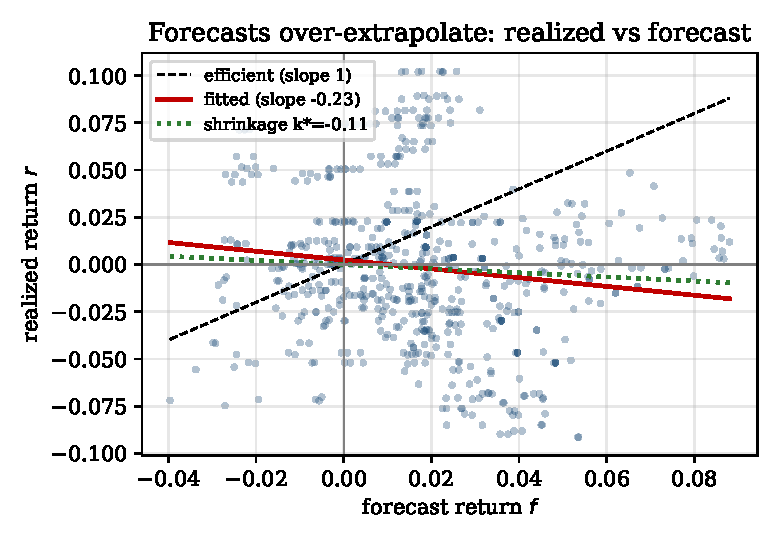
\includegraphics[width=0.60\textwidth]{fig_mz_scatter.pdf}
\caption{Realized return $r$ versus forecast return $f$ for the $619$ resolved
forecasts. The fitted Mincer--Zarnowitz line (slope $-0.23$) tilts opposite to the
$45^\circ$ efficient line; the dotted line is the error-minimizing shrinkage
$k^\star$. Bold forecasts are followed by reversal --- the more the model predicts, the
more the realized return disappoints.}
\label{fig:mz}
\end{figure*}

\subsection{Over-extrapolation, made visible}
A negative efficiency slope is the global signature of over-extrapolation; the local
picture confirms it. Binning forecasts into sextiles of $f_t$ and reading off the mean
realized return in each bin gives a reliability curve for the point forecast
(\fig{rel}). The curve is flat-to-inverted at the extremes: the most bullish sextile,
with mean forecast $+5.5\%$, realizes $-1.3\%$ on average; the next, with mean forecast
$+3.0\%$, realizes $-2.2\%$. Only the timid middle bins, where the forecast barely
commits, sit near the diagonal. Directional accuracy --- the rate at which
$\operatorname{sign}(f_t)=\operatorname{sign}(r_t)$ --- is $0.464$, below a coin. The
forecaster is most wrong precisely where it is most confident, the point-forecast
counterpart of the over-confidence that plagues deployed predictors generally.

\begin{figure}[!t]
\centering
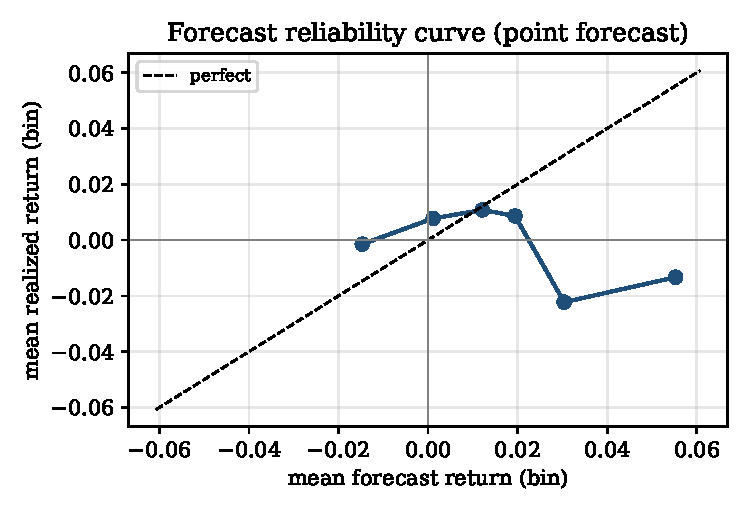
\includegraphics[width=0.92\linewidth]{fig_reliability_point.pdf}
\caption{Reliability curve of the point forecast: mean realized return against mean
forecast return within sextiles of $f$. A perfectly efficient forecaster would lie on
the diagonal. The confident (high-$|f|$) bins fall below zero --- bold forecasts
reverse.}
\label{fig:rel}
\end{figure}

\tab{sextile} gives the numbers behind the curve. The first four sextiles, spanning
forecasts from $-1.5\%$ to $+1.9\%$, track realized returns loosely and with
hit-rates near a half. The damage is in the top two: sextile S5 (mean forecast
$+3.0\%$) realizes $-2.2\%$ with a directional hit-rate of just $27\%$, and S6 (mean
forecast $+5.5\%$) realizes $-1.3\%$. Almost all of the negative efficiency slope is
manufactured by the forecasts in which the model is most committed, which is exactly
the regime in which a user would lean on it hardest.

\begin{table}[!t]
\footnotesize
\centering
\caption{Over-extrapolation by forecast sextile: mean forecast return, mean realized
return, and directional hit-rate. The two most confident sextiles reverse.}
\label{tab:sextile}
\vspace{2pt}
\begin{tabular}{lrrrr}
\toprule
Sextile & $n$ & mean $f$ & mean $r$ & hit-rate \\
\midrule
S1 (most bearish) & $103$ & $-1.5\%$ & $-0.2\%$ & $0.53$ \\
S2 & $103$ & $+0.1\%$ & $+0.8\%$ & $0.48$ \\
S3 & $103$ & $+1.2\%$ & $+1.1\%$ & $0.56$ \\
S4 & $103$ & $+1.9\%$ & $+0.9\%$ & $0.52$ \\
S5 & $103$ & $+3.0\%$ & $-2.2\%$ & $0.27$ \\
S6 (most bullish) & $104$ & $+5.5\%$ & $-1.3\%$ & $0.41$ \\
\bottomrule
\end{tabular}
\end{table}

\subsection{Decomposing the error}
\label{sec:theil}
Where does the forecast's error come from? Theil's decomposition splits the
mean-squared error into three proportions that sum to one --- a bias term
$U^M=(\bar f-\bar r)^2/\mathrm{MSE}$, a variance term $U^S=(s_f-s_r)^2/\mathrm{MSE}$,
and a covariance (disturbance) term $U^C=2(1-\rho)s_f s_r/\mathrm{MSE}$ --- and compares
the forecast against a naive no-change benchmark through the inequality coefficient
$U_2=\mathrm{RMSE}_{\text{forecast}}/\mathrm{RMSE}_{\text{no-change}}$ \cite{theil1966}.
On the full sample (\tab{theil}) the bias proportion is $0.13$ and the variance
proportion $0.11$: the forecasts are systematically too optimistic (mean $+1.7\%$
against a realized $-0.2\%$) and too smooth (standard deviation $2.3\%$ against a
realized $4.1\%$), so they shrink the cross-section of outcomes toward a rosy centre.
The decisive number is $U_2=1.30>1$: the forecast's RMSE is $30\%$ \emph{larger} than
that of a forecaster who simply predicts no change. A forecast that loses to no-change
on its own error metric, before any efficiency test, is already a candidate for the
shrinkage we now make precise.

\begin{table}[!t]
\footnotesize
\centering
\caption{Theil decomposition of the forecast's mean-squared error and inequality
coefficient $U_2$ (full sample). $U_2>1$ means worse than a no-change benchmark.}
\label{tab:theil}
\vspace{2pt}
\begin{tabular}{lr}
\toprule
Quantity & Value \\
\midrule
Bias proportion $U^M$        & $0.13$ \\
Variance proportion $U^S$    & $0.11$ \\
Covariance proportion $U^C$  & $0.76$ \\
Theil $U_2$ (vs.\ no-change) & $1.30$ \\
\bottomrule
\end{tabular}
\end{table}

% =============================================================================
\section{The Shrinkage Correction}
\label{sec:shrink}
% =============================================================================
The efficiency failure has an immediate, optimal, one-parameter remedy. Consider the
family of linear forecasts $\tilde f_t(k) = k\,f_t$ and choose $k$ to minimize expected
squared error. The minimizer is the projection coefficient
\begin{equation}
k^\star = \frac{\sum_t f_t\, r_t}{\sum_t f_t^{2}},
\label{eq:kstar}
\end{equation}
which is exactly the (no-intercept) regression slope of $r_t$ on $f_t$ and therefore
inherits the sign of the efficiency slope. A forecast that passes the efficiency test
has $k^\star=1$ (leave it alone); a pure-noise forecast has $k^\star=0$ (discard it);
a perversely-signed forecast has $k^\star<0$ (use its opposite). Estimated on the
calibration window, $k^\star = -0.11$, with a bootstrap $95\%$ interval of
$[-0.33,0.09]$ that \emph{contains zero}.

\begin{proposition}[Discard-the-arrow]
If the error-minimizing shrinkage $k^\star$ is not statistically distinguishable from
$0$, then the drift forecast $\tilde f_t\equiv \bar r$ (here $\bar r\approx 0$) is,
up to estimation error, the minimum-MSE member of the family $\{k f_t\}$, and the
forecast's directional content carries no usable information. The optimal deployment
is to predict the drift and route the forecast's direction nowhere.
\end{proposition}

\noindent The proposition is not a claim that the forecasts are random --- their slope
is significantly negative --- but a claim about \emph{action}: because $k^\star$ cannot be
pinned away from zero on the available sample, betting on the small negative slope is
not warranted, and the safe, error-minimizing operating point is plain drift. We
deliberately resist the more aggressive reading (``trade the system contrarian,''
$k<0$): the contrarian edge, if real, is too small relative to its estimation error and
to transaction costs to deploy, and claiming it would repeat exactly the
over-confidence we are studying. The honest output of the analysis is the degenerate
shrinkage, not a new alpha.

% =============================================================================
\section{Out-of-Sample Evaluation}
\label{sec:results}
% =============================================================================
\subsection{Protocol}
Forecasts are ordered by issue time and split $60/40$ into a past calibration window
($371$ forecasts), on which $k^\star$ is estimated, and a future test window ($248$
forecasts), on which all errors are reported. The comparison is therefore strictly
walk-forward. We evaluate three forecasts on the test window: the raw forecast $f_t$;
the optimally shrunk forecast $k^\star f_t$; and the drift baseline $0$ (predict no
excess move). We report root-mean-square error, mean absolute error, and
Diebold--Mariano tests of equal squared-error loss with a Newey--West long-run variance
\cite{diebold1995}.

\subsection{Results}
\tab{oos} collects the numbers and \fig{rmse} shows the error bars. The raw forecast
has out-of-sample RMSE $0.0534$. Shrinking to the drift baseline cuts it to $0.0307$,
and the optimally-shrunk forecast reaches $0.0299$ --- reductions of $67\%$ and $69\%$
in mean-squared error, respectively. The pattern in MAE is identical ($0.042 \to 0.022$).
The Diebold--Mariano statistic for raw versus drift is $6.4$ and for raw versus
optimally-shrunk is $6.2$: both corrections beat the raw forecast far beyond any
conventional significance threshold. Crucially, the statistic for drift versus
optimally-shrunk is only $1.8$ --- not significant --- so the data cannot distinguish the
plain drift baseline from the optimally tuned shrinkage. The simplest correction is, on the
evidence, the best one.

\begin{table}[!t]
\footnotesize
\centering
\caption{Out-of-sample forecast error on the held-out test window ($248$ forecasts).
DM is the Diebold--Mariano statistic against the raw forecast (squared-error loss,
Newey--West variance); larger means a more significant improvement over raw.}
\label{tab:oos}
\vspace{2pt}
\begin{tabular}{lcccc}
\toprule
Forecast & RMSE & MAE & MSE red.\ vs raw & DM vs raw \\
\midrule
Raw $f_t$               & $0.0534$ & $0.0423$ & ---     & ---  \\
Affine $a+b f_t$        & $0.0314$ & $0.0231$ & $65\%$  & --- \\
Drift ($0$)             & $0.0307$ & $0.0225$ & $67\%$  & $6.4$ \\
Shrunk $k^\star f_t$    & $0.0299$ & $0.0223$ & $69\%$  & $6.2$ \\
\bottomrule
\end{tabular}
\end{table}

\begin{figure}[!t]
\centering
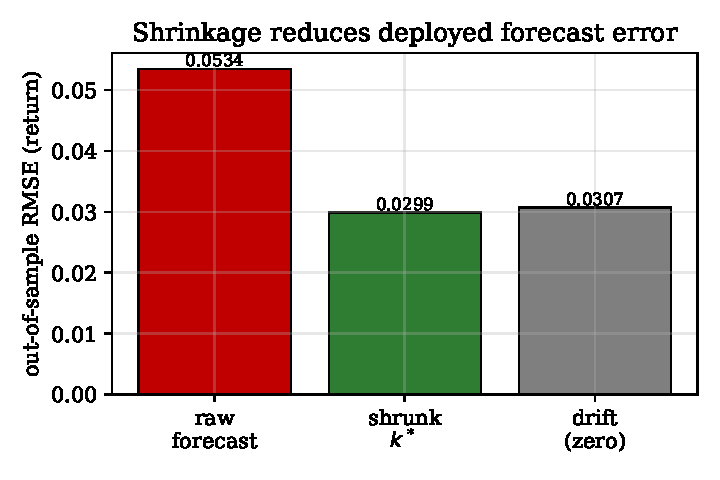
\includegraphics[width=0.86\linewidth]{fig_oos_rmse.pdf}
\caption{Out-of-sample RMSE of the raw forecast, the optimally-shrunk forecast, and the
drift baseline. Discarding the forecast's directional content (drift) recovers almost
all of the achievable error reduction.}
\label{fig:rmse}
\end{figure}

A two-parameter affine recalibration $a+b f_t$, fitted on the calibration window
($\hat a=0.007$, $\hat b=-0.25$) and applied walk-forward, lands at RMSE $0.0314$
(\tab{oos}) --- between drift and the optimal shrinkage and, like them, far better than
raw, but no better than simply predicting drift. The extra free parameter, which would
turn the system mildly contrarian, buys nothing the data can certify. This reinforces
the proposition of \refsec{shrink}: once the forecast's directional content is removed,
there is little left to recalibrate, and the drift baseline is the honest endpoint.

\subsection{Robustness and heterogeneity}
\label{sec:robust}
The negative efficiency slope is stable to several perturbations and, in one important
respect, is not. Restricting to the dominant ten-day horizon leaves
$\hat b=-0.21$ (s.e.\ $0.07$, $n=573$); winsorizing forecast and realized returns at
the $2.5$/$97.5$ percentiles --- so that no single extreme observation drives the fit ---
gives $\hat b=-0.25$. Splitting by forecast sign, the $472$ bullish forecasts (mean
$+2.6\%$) realize $-0.25\%$ on average with only a $46\%$ chance of a positive return,
and the $147$ bearish forecasts realize $+0.10\%$; both signs are mildly
anti-informative. So the aggregate inefficiency is neither a horizon artifact nor an
outlier artifact.

It is, however, \emph{not uniform across instruments}, and we report this plainly. A
leave-one-instrument-out jackknife of the slope (\tab{jack}) shows that two names,
RELIANCE and TCS, supply most of the negative relationship: dropping RELIANCE flips the
slope to $+0.27$, while dropping TCS deepens it to $-0.51$. The over-extrapolation is
therefore concentrated rather than universal. We draw two conclusions. First, the
\emph{system-level} verdict stands: the deployed forecaster, as it actually emits
forecasts across its universe, has a significantly negative aggregate efficiency slope,
and shrinking its aggregate output to drift improves aggregate out-of-sample error.
Second, the right long-run fix is per-instrument: the same analysis, run name-by-name as
the ledger grows, will re-enable the directional signal for instruments whose slope is
reliably positive and suppress it for those whose slope is reliably negative. On the
present sample the per-instrument slopes are too noisy to act on individually, which is
why we recommend the aggregate drift rule as the current operating point and the
per-instrument analysis as the maintenance procedure.

\begin{table}[!t]
\footnotesize
\centering
\caption{Leave-one-instrument-out jackknife of the Mincer--Zarnowitz slope. The
aggregate slope ($-0.23$) is concentrated in a subset of instruments.}
\label{tab:jack}
\vspace{2pt}
\begin{tabular}{lrr}
\toprule
Instrument removed & $n$ remaining & slope $\hat b$ \\
\midrule
HDFCBANK  & $556$ & $-0.27$ \\
ICICIBANK & $556$ & $-0.24$ \\
INFY      & $556$ & $-0.22$ \\
SBIN      & $610$ & $-0.23$ \\
RELIANCE  & $298$ & $+0.27$ \\
TCS       & $519$ & $-0.51$ \\
\midrule
\emph{none (full sample)} & $619$ & $-0.23$ \\
\bottomrule
\end{tabular}
\end{table}

% =============================================================================
\section{Discussion}
\label{sec:discussion}
% =============================================================================
The procedure we followed is compact enough to state as a reusable recipe
(Algorithm~\ref{alg:analysis}); it presumes only that forecasts were recorded before their
outcomes and costs nothing beyond two regressions and a paired test.

\begin{algorithm}[!t]
\caption{Efficiency analysis and shrinkage correction}
\label{alg:analysis}
\begin{algorithmic}[1]
\STATE \textbf{Input:} point-in-time ledger of forecast/realized pairs $\{(f_t,r_t)\}$,
level $\alpha$, time split $\tau$
\STATE Fit $r=a+bf$ on all pairs; report $\hat b$ and a bootstrap interval
\IF{interval for $\hat b$ excludes $1$}
  \STATE flag the forecast as \emph{inefficient}
\ENDIF
\STATE On $t\le\tau$ estimate $k^\star=\sum f_t r_t/\sum f_t^2$ and a bootstrap interval
\IF{interval for $k^\star$ contains $0$}
  \STATE deploy the drift forecast $\bar r$; route the point direction nowhere
\ELSE
  \STATE deploy $k^\star f_t$
\ENDIF
\STATE On $t>\tau$ confirm by Diebold--Mariano that the deployed choice beats raw
\STATE \textbf{Re-run} per-instrument as the ledger grows
\end{algorithmic}
\end{algorithm}

\textbf{What the analysis changes in deployment.} The practical output is a routing
decision. A deployed forecasting service typically emits several signals --- a point
direction, a magnitude, an uncertainty band, an abstention flag. Our analysis says that on
this system the point \emph{direction} should be cut from the decision path entirely,
because it is significantly anti-informative and its optimal weight is indistinguishable
from zero, while the drift and the calibrated uncertainty remain useful. This is a
cheaper and safer intervention than retraining, and it is reversible: should a later,
larger ledger show $k^\star$ moving significantly away from zero, the same analysis will
detect it and re-enable the signal.

\textbf{Why accuracy metrics hid the problem.} The raw forecast's median magnitude
($1.7\%$) is plausible and its RMSE ($5.3\%$) is unremarkable for ten-day equity
returns; a dashboard reporting only these would raise no alarm. The efficiency test is
what exposes that the forecast's \emph{ordering} of outcomes is inverted. We therefore
argue that any deployed point forecaster should report a Mincer--Zarnowitz slope and a
directional-accuracy figure alongside its error magnitudes, because the latter can be
acceptable while the former is catastrophic. An efficiency slope is as cheap to compute
as an RMSE and far more diagnostic of whether the forecast should be acted upon.

\subsection{A minimal reporting standard}
\label{sec:reporting}
The analysis suggests a small reporting standard that any deployed point forecaster could
adopt at negligible cost. Alongside the usual error magnitudes, we recommend reporting
four diagnostics, each a one-line computation over the same ledger and each carrying an
explicit red flag:
\begin{enumerate}
\item the Mincer--Zarnowitz slope $\hat b$ with a confidence interval, flagged when the
interval excludes $1$;
\item directional accuracy, flagged when it falls below one half;
\item Theil's inequality coefficient $U_2$ against the no-change benchmark, flagged when
it exceeds $1$;
\item a Diebold--Mariano comparison of the forecast against the drift baseline, flagged
when drift is not beaten.
\end{enumerate}
On the system studied here all four flags fire. Any one of them, watched in production,
would have caught the failure long before a position depended on it. The value of a
standard is that it fires automatically: a team need not suspect a problem to find it,
because the diagnostics are recomputed every period and the flags raise themselves. None
of the four needs labels beyond the realized outcome the ledger already stores, and none
requires re-running the model, so the standard adds a few lines of analysis rather than
any new infrastructure.

\textbf{Consistency with market efficiency.} A significantly negative single-name
efficiency slope does not contradict near-market-efficiency \cite{fama1970,welch2008};
it is what one expects when an over-extrapolating model is pitted against a target that
is close to a martingale. The model manufactures conviction the market does not reward,
and the conviction reverts. The corrective --- shrink to the drift --- is the operational
statement of ``do not bet against the martingale on noise.''

\subsection{From analysis to routing: a general principle}
\label{sec:routing}
The specific verdict --- discard this system's directional content --- generalizes to a
maintenance principle for any deployed forecaster that emits several signals into a
decision. Each signal carries an implicit efficiency claim, and each can be evaluated the
same way: regress the realized target on the signal, test the slope, and weight the
signal by the error-minimizing coefficient, defaulting to its prior when the
coefficient cannot be separated from zero. A decision layer assembled from such studied
weights degrades gracefully: a signal that loses its information --- through regime
change, data-feed decay, or model staleness --- has its weight pulled toward zero by the
next analysis rather than silently corrupting the decision. The append-only ledger makes
this loop cheap, because the analysis is a deterministic recomputation over the same
immutable records that already exist for accountability. We therefore see the
contribution less as a one-off finding about one model and more as an instance of a
routing discipline: \emph{trust each signal exactly as far as its out-of-sample
efficiency, re-measured continuously, allows} --- and let the drift, the cheapest and
most robust signal of all, absorb whatever weight the others cannot earn.

\textbf{Why not simply retrain?} Retraining presumes the inefficiency is a fixable
modeling defect rather than a property of a near-efficient target. On a martingale-like
series, a more powerful model fit to the same features will tend to manufacture the same
over-extrapolation, and a model selected on in-sample fit will do so more confidently.
The analyze-and-shrink approach is conservative by design: it neither assumes an edge exists
nor destroys one if it does, because the shrinkage coefficient is re-estimated from data
and will rise above zero exactly when, and only when, the signal earns it.

% =============================================================================
\section{Threats to Validity and Reproducibility}
\label{sec:threats}
% =============================================================================
\textbf{Scope.} Six instruments, eight weeks, one regime. The specific numbers ---
slope, $k^\star$, error reductions --- are properties of this ledger and may differ
elsewhere; we make no cross-market claim. What we do claim to be general is the
\emph{method} and the warning it embodies. \textbf{Stationarity.} The efficiency
regression and the shrinkage assume the forecast--realization relationship is stable
enough across the calibration and test windows; we mitigate this by reporting
walk-forward errors on a strictly later window rather than in-sample fits, and the
out-of-sample improvement confirms the relationship held over the test period.
\textbf{Choice of loss.} The shrinkage optimum $k^\star$ and the Diebold--Mariano
comparison are stated for squared-error loss, the loss under which the conditional mean
is the optimal forecast and the Mincer--Zarnowitz test is the natural diagnostic. A user
whose decisions imply an asymmetric or piecewise-linear loss would re-derive the optimal
transform under that loss; the analysis procedure is unchanged, only the projection in
\eqref{eq:kstar} is replaced by the corresponding loss-specific minimizer. We report
squared error because it is the default for point-forecast evaluation and because it is
the loss against which the deployed forecaster's own training objective is most
charitably interpreted; the qualitative verdict --- a negative efficiency slope --- is a
property of the sign of $\sum_t f_t r_t$ and does not depend on the loss at all.

\textbf{Estimation risk in $k^\star$.} We treat $k^\star$ as indistinguishable from
zero precisely because its bootstrap interval straddles zero; we do not deploy the point
estimate. \textbf{Reproducibility.} Every figure and number is a deterministic function
of the immutable ledger: the Mincer--Zarnowitz fit, the bootstrap intervals (fixed
seed), the fixed $60/40$ time split, the shrinkage coefficient, and the
Diebold--Mariano statistics are all recomputed by a single script. The append-only,
point-in-time ledger is the reusable artifact, and the method transfers unchanged to any
forecaster that records its predictions before the outcome is known.

% =============================================================================
\section{Conclusion}
\label{sec:conclusion}
% =============================================================================
We studied the point forecasts of a deployed equity-return forecaster on a leakage-free
ledger and found them inefficient to the point of inversion: a Mincer--Zarnowitz slope
of $-0.23$ (interval $[-0.35,-0.12]$), directional accuracy of $46.4\%$, and a
reliability curve in which the boldest forecasts reverse. The error-minimizing correction is
a scalar shrinkage whose optimum is statistically indistinguishable from zero, so the
right deployment action is to discard the forecast's directional content and predict the
drift --- which cuts out-of-sample error by two-thirds and is, by a Diebold--Mariano test,
as good as anything the data support. Beyond the specific system, the message is a
discipline: report and act on forecast \emph{efficiency}, not just forecast error,
because a model can be confidently, plausibly, and significantly wrong in a way that only
the efficiency test reveals. Discard the arrow; keep the drift.

% =============================================================================
\section*{Acknowledgment}
% =============================================================================
Generative AI assistance was used for language editing and for drafting the analysis and
figure-generation scripts. All quantitative results were computed by the authors'
deterministic code directly from the deployment ledger and verified by the authors; no
numerical result, table, or figure was produced by a language model.

% =============================================================================
\begin{thebibliography}{99}

\bibitem{mincer1969} J.~Mincer and V.~Zarnowitz, ``The evaluation of economic
forecasts,'' in \emph{Economic Forecasts and Expectations}, J.~Mincer, Ed.\ New York:
NBER, 1969, pp.\ 3--46.

\bibitem{theil1966} H.~Theil, \emph{Applied Economic Forecasting}. Amsterdam:
North-Holland, 1966.

\bibitem{diebold1995} F.~X. Diebold and R.~S. Mariano, ``Comparing predictive
accuracy,'' \emph{Journal of Business \& Economic Statistics}, vol.\ 13, no.\ 3,
pp.\ 253--263, 1995.

\bibitem{bordalo2018} P.~Bordalo, N.~Gennaioli, and A.~Shleifer, ``Diagnostic
expectations and credit cycles,'' \emph{Journal of Finance}, vol.\ 73, no.\ 1,
pp.\ 199--227, 2018.

\bibitem{bordalo2019} P.~Bordalo, N.~Gennaioli, Y.~Ma, and A.~Shleifer,
``Over-reaction in macroeconomic expectations,'' \emph{American Economic Review},
vol.\ 110, no.\ 9, pp.\ 2748--2782, 2020.

\bibitem{greenwood2014} R.~Greenwood and A.~Shleifer, ``Expectations of returns and
expected returns,'' \emph{Review of Financial Studies}, vol.\ 27, no.\ 3,
pp.\ 714--746, 2014.

\bibitem{fama1970} E.~F. Fama, ``Efficient capital markets: a review of theory and
empirical work,'' \emph{Journal of Finance}, vol.\ 25, no.\ 2, pp.\ 383--417, 1970.

\bibitem{welch2008} I.~Welch and A.~Goyal, ``A comprehensive look at the empirical
performance of equity premium prediction,'' \emph{Review of Financial Studies},
vol.\ 21, no.\ 4, pp.\ 1455--1508, 2008.

\bibitem{campbell2008} J.~Y. Campbell and S.~B. Thompson, ``Predicting excess stock
returns out of sample: can anything beat the historical average?'' \emph{Review of
Financial Studies}, vol.\ 21, no.\ 4, pp.\ 1509--1531, 2008.

\bibitem{gu2020} S.~Gu, B.~Kelly, and D.~Xiu, ``Empirical asset pricing via machine
learning,'' \emph{Review of Financial Studies}, vol.\ 33, no.\ 5, pp.\ 2223--2273,
2020.

\bibitem{bailey2014} D.~H. Bailey, J.~Borwein, M.~L\'opez de Prado, and Q.~J. Zhu,
``Pseudo-mathematics and financial charlatanism: the effects of backtest overfitting
on out-of-sample performance,'' \emph{Notices of the AMS}, vol.\ 61, no.\ 5,
pp.\ 458--471, 2014.

\bibitem{lopez2018} M.~L\'opez de Prado, \emph{Advances in Financial Machine
Learning}. Hoboken, NJ: Wiley, 2018.

\bibitem{stein1956} C.~Stein, ``Inadmissibility of the usual estimator for the mean of
a multivariate normal distribution,'' in \emph{Proc.\ 3rd Berkeley Symp.\ on
Mathematical Statistics and Probability}, vol.\ 1, 1956, pp.\ 197--206.

\bibitem{james1961} W.~James and C.~Stein, ``Estimation with quadratic loss,'' in
\emph{Proc.\ 4th Berkeley Symp.\ on Mathematical Statistics and Probability}, vol.\ 1,
1961, pp.\ 361--379.

\bibitem{hoerl1970} A.~E. Hoerl and R.~W. Kennard, ``Ridge regression: biased
estimation for nonorthogonal problems,'' \emph{Technometrics}, vol.\ 12, no.\ 1,
pp.\ 55--67, 1970.

\bibitem{timmermann2006} A.~Timmermann, ``Forecast combinations,'' in \emph{Handbook of
Economic Forecasting}, vol.\ 1, G.~Elliott, C.~Granger, and A.~Timmermann, Eds.\
Amsterdam: Elsevier, 2006, pp.\ 135--196.

\end{thebibliography}

\end{document}
